\subsection{Comparison with the reference estimators}
\label{sec:comparacao_referencias}

On clean light, GATv2-cascade has a mean 3-D error \qty{1.71}{\cm} lower than that of XGBoost (\num{0.83} to \qty{2.62}{\cm}) and a combined RMSE \qty{2.30}{\cm} lower (\num{1.66} to \qty{2.95}{\cm}); against LightGBM, \num{1.91} and \qty{1.98}{\cm} (Figure~\ref{fig:diferenca_pareada} and Table~\ref{tab:referencias}). By the point estimates, seven of the \num{11} encoders have a mean 3-D error lower than that of XGBoost, but GATv2-cascade lands closer to the vertex than XGBoost in only \qty{47.6}{\percent} of the events: XGBoost errs less on the brightest events, and GATv2-cascade on the dimmest ones and in the tail, with the 90th percentile of the \mbox{3-D} error at \qty{51.26}{\cm} against \qty{60.26}{\cm} (Section~\ref{sec:onde_erro}). In the run records, on augmented light, XGBoost has a mean MAE of \qty{13.01}{\cm} and a combined RMSE of \qty{20.82}{\cm}, against \num{13.21} and \qty{20.95}{\cm} on clean light.

Compared with the network of the previous stage \citep{vicentin2024study}, with values obtained on a different partition and in the geometry prior to the corrections, the combined RMSE of GATv2-cascade is \qty{10.6}{\percent} lower (\num{18.64} against \qty{20.86}{\cm}) and its mean MAE \qty{16.5}{\percent} lower (\num{12.63} against \qty{15.13}{\cm}). Per axis, in the sensor frame, the RMSE falls by \num{4.23} and \qty{1.81}{\cm} in $x$ and $y$, and in $z$ the value of that network, \qty{0.41}{\cm} higher, lies within the \qty{95}{\percent} interval of GATv2-cascade. On clean light, the boosters lie within \qty{0.24}{\cm} of the combined RMSE of that network, and the \num{11} encoders lie below it, between \num{18.55} and \qty{20.64}{\cm}; for EdgeConv, GINE and GINE-cascade, as for the boosters, the value of that network lies within the \qty{95}{\percent} interval.

\begin{table}[H]
  \centering
  \caption{Test errors of GATv2-cascade, GPS and the reference estimators, in cm, in the sensor frame; the barycentre has a quadratic calibration. \textsuperscript{a}Quoted per-axis RMSE values, from a different partition (\qty{80}{\percent} and \qty{20}{\percent}) and from the geometry prior to the corrections \citep{vicentin2024study}, with the axes converted to this frame; combined RMSE and mean MAE computed from the published per-axis values. \textsuperscript{\smash{b}}A different simulation \citep{marinho2025apex}; widths read from Figure~2 of the paper at \qty{0.26}{\cm} per pixel, at equal detected light with the average yield (\qty{2.9}{\MeV}) or with the minimum (\qty{4.9}{\MeV}) and at equal energy (\qty{10}{\MeV}); the two transverse widths appear in the same cell, without assignment to $x$ and $y$; MAE not available.}
  \label{tab:referencias}
  \begin{tabular}{@{}l S[table-format=2.2] S[table-format=2.2] S[table-format=2.2] S[table-format=2.2] S[table-format=2.2]@{}}
\toprule
 & {RMSE $x$} & {RMSE $y$} & {RMSE $z$} & {RMSE} & {Mean} \\
Estimator & {(cm)} & {(cm)} & {(cm)} & {comb.\ (cm)} & {MAE (cm)} \\
\midrule
GATv2-cascade & 20.45 & 14.35 & 20.46 & 18.64 & 12.63 \\
GPS & 20.55 & 14.29 & 20.15 & 18.55 & 12.95 \\
\midrule
XGBoost, clean light & 23.82 & 16.96 & 21.47 & 20.95 & 13.21 \\
LightGBM, clean light & 23.91 & 16.55 & 20.75 & 20.62 & 13.38 \\
Barycentre ($z$ only) &  &  & 42.45 &  &  \\
\midrule
Dense network (2024)\textsuperscript{a} & 24.68 & 16.16 & 20.87 & 20.86 & 15.13 \\
APEX, \qty{2.9}{\MeV}\textsuperscript{b} & \multicolumn{2}{c}{\num{33.1} and \num{51.3}} & 24.8 & 38.0 &  \\
APEX, \qty{4.9}{\MeV}\textsuperscript{b} & \multicolumn{2}{c}{\num{26.8} and \num{44.0}} & 19.4 & 31.8 &  \\
APEX, \qty{10}{\MeV}\textsuperscript{b} & \multicolumn{2}{c}{\num{20.8} and \num{37.3}} & 13.7 & 25.9 &  \\
\bottomrule
\end{tabular}

\end{table}

At detected light equal to the test mean and with the average yield, the combined width of APEX \citep{marinho2025apex} is \qty{38.0}{\cm}, and the combined RMSE of GATv2-cascade, \qty{18.64}{\cm} (\num{17.69} to \qty{19.61}{\cm}), is \qty{51.0}{\percent} lower; with the minimum yield, it is \qty{41.3}{\percent} lower than the width of \qty{31.8}{\cm}, and at equal energy, \qty{28.0}{\percent} lower than that of \qty{25.9}{\cm} (Figure~\ref{fig:apex_luz}). In $z$, against \num{20.15} to \qty{20.46}{\cm} for the four best, APEX has \qty{24.8}{\cm} with the average yield, above the \qty{95}{\percent} interval of each of them, and \qty{19.4}{\cm} with the minimum, within it; only at equal energy (\qty{13.7}{\cm}) is it better. The paper does not define the width: at \qty{4}{\MeV}, the plotted value is \num{0.96} times the standard deviation and \num{1.13} times the Gaussian width of the residuals in $z$; a Gaussian width, smaller than the standard deviation, would favour APEX against an RMSE.

{\clubpenalty=10000 On the same events, the barycentre $\bar{z}$ \citep{marinho2025apex}, here with a quadratic calibration, has an RMSE in $z$ of \qty{42.45}{\cm} (\num{39.55} to \qty{45.22}{\cm}; \qty[uncertainty-mode = separate, separate-uncertainty-units = single]{41.98 \pm 0.61}{\cm}, mean and standard deviation over \num{30} photon draws; Figure~\ref{fig:baricentro_luz}), \num{2.07} times that of GATv2-cascade, and with a cubic calibration, \qty{41.86}{\cm}. Without calibration, the barycentre has \qty{66.59}{\cm}, shifted on average by \qty{34.08}{\cm} towards the nearest end cap, mainly for the vertices from $z = {}$\qty{20}{\m} upwards (Section~\ref{sec:onde_erro}), a bias not found in APEX. Of the single-statistic estimators tested, the barycentre of all channels is the best (with a cubic calibration, barycentre of only the channels more than \qty{1}{\m} from the end caps: \qty{66.95}{\cm}; brightest channel: \qty{142.16}{\cm}).\par}

\begin{figure}[H]
  \centering
  \begin{subfigure}[t]{0.485\textwidth}
    \centering
    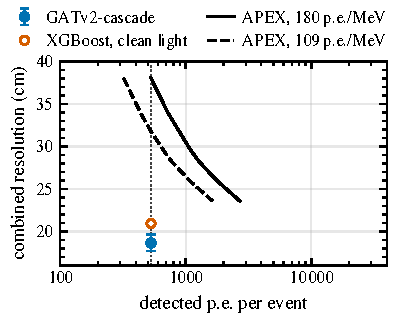
\includegraphics{figures/apex_luz.pdf}
    \caption{Combined width of APEX in a different simulation \citep{marinho2025apex}, with the energy converted into photoelectrons by the average yield (\qty{180}{\pe\per\MeV}; \qty{10}{\MeV} gives \qty{1800}{\pe}) and by the minimum (\qty{109}{\pe\per\MeV}), and the combined RMSE of GATv2-cascade (\qty{95}{\percent} interval) and of \mbox{XGBoost} on clean light, at the mean test light (\qty{530.1}{\pe}, dotted line).}
    \label{fig:apex_luz}
  \end{subfigure}\hfill
  \begin{subfigure}[t]{0.485\textwidth}
    \centering
    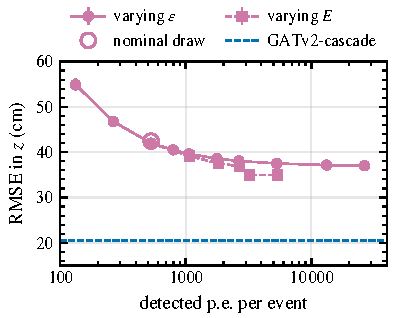
\includegraphics{figures/baricentro_luz.pdf}
    \caption{RMSE in $z$ of the barycentre with a quadratic calibration, on the test set, varying the efficiency $\varepsilon$ from \num{0.005} to \num{1}, with $E$ fixed at \qty{10}{\MeV}, or the energy $E$ from \num{10} to \qty{100}{\MeV}, with $\varepsilon$ fixed at \num{0.02}: mean over \num{30} photon draws and standard deviation (bars, smaller than the markers except at $\varepsilon = {}$\num{0.005}); hollow circle: nominal draw, used for training and testing the models; horizontal line: GATv2-cascade, evaluated on that draw only.}
    \label{fig:baricentro_luz}
  \end{subfigure}
  \caption{Resolution as a function of the detected light per event, for the analytic estimators and, at the test light only, for the models: (a) combined over the three axes; (b) in $z$.}
  \label{fig:par_luz_referencias}
\end{figure}
